\section{Ejemplos introductorios}
\subsection{Problema de programación lineal de dos incógnitas (en $\R^2$)}
\begin{ejem} Veamos a continuación un ejemplo de problema de programación lineal.\\

Una empresa fabrica dos tipos de productos: A y B. Los productos A y B generan unos beneficios de 100 y 600 euros respectivamente. La empresa no puede fabricar más de 4 productos diarios y además sólo recibe material suficiente para fabricar a lo sumo 2 productos A y 3 productos B al día. Veamos cuál es el beneficio máximo de la empresa a diario.\\

Planteemos el problema. Tenemos:\\
Función objetivo:
\[\mathrm{m\acute{a}x}\ z = 100x_1 + 600x_2\]
Restricciones:
\[x_1\leq 2\]
\[x_2\leq 3\]
\[x_1+x_2\leq 4\]
\[x_1,x_2\geq 0\]
No es difícil darse cuenta que cada restricción define una inecuación lineal en el plano generado por $\R^2$ que a su vez designa una parte del plano que satisface cada inecuación. Luego la región factible de este problema, si la hay, será la intersección de las partes del plano designadas por cada inecuación, como podemos observar en la \textit{figura 2.1}.
\begin{figura}\ \begin{center} \definecolor{zzttqq}{rgb}{0.6,0.2,0.}
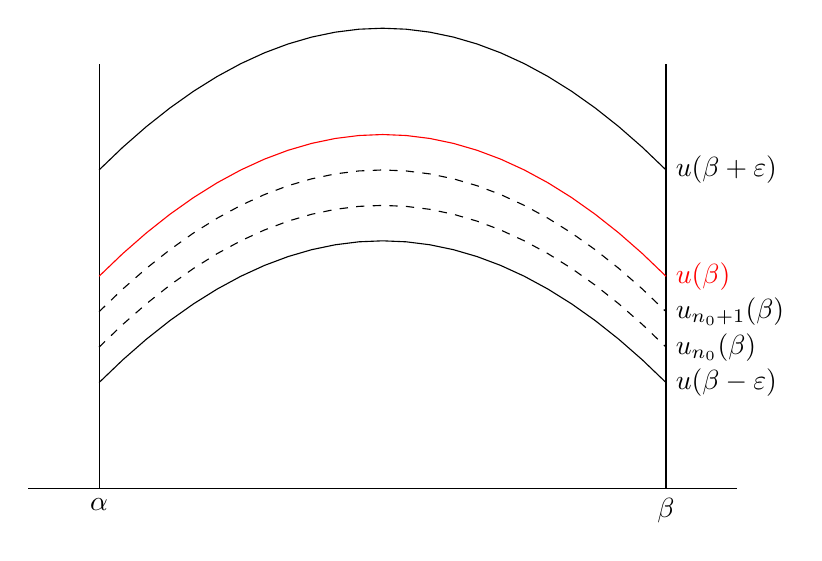
\begin{tikzpicture}[x=0.9cm,y=0.9cm]
\draw[color=black] (-1,0) -- (9,0);
\draw[color=black] (0,0) -- (0,6);
\draw[color=black] (8,0) -- (8,6);
\draw [domain=0:8, color=red] plot(\x,{-(1/8)*\x*\x+\x+3});
\draw [domain=0:8] plot(\x,{-(1/8)*\x*\x+\x+4.5});
\draw [domain=0:8] plot(\x,{-(1/8)*\x*\x+\x+1.5});
\draw [domain=0:8, dashed] plot(\x,{-(1/8)*\x*\x+\x+2.5});
\draw [domain=0:8, dashed] plot(\x,{-(1/8)*\x*\x+\x+2});
\draw[color=red] (8,3) node[anchor=west] {$u(\beta)$};
\draw (8,4.5) node[anchor=west] {$u(\beta+\varepsilon)$};
\draw (8,1.5) node[anchor=west] {$u(\beta-\varepsilon)$};
\draw (8,2) node[anchor=west] {$u_{n_0}(\beta)$};
\draw (8,2.5) node[anchor=west] {$u_{n_0+1}(\beta)$};
\draw (0,0) node[anchor=north] {$\alpha$};
\draw (8,0) node[anchor=north] {$\beta$};


\end{tikzpicture}\end{center} \end{figura}
Además, supongamos un valor $c$ fijo tal que $z(x_1,x_2)=c \iff 100x_1+600x_2=c\iff\\
\iff x_2=\dfrac{c-100x_1}{600}$, luego para cada valor $c$ que puede tomar la función $z$ tenemos otra ecuación lineal que define una recta de nivel. En dicha recta, cada par de puntos $x_1,x_2$ de la misma genera un mismo valor $c$ para nuestra función objetivo. Por lo tanto podemos trazar rectas paralelas para distintos valores de $c$ tal y como se muestra en la \textit{figura 2.2} para intuir cual es el punto donde encontramos la solución óptima (máximo) de nuestra función.
\newpage
\begin{figura}\ \begin{center}\definecolor{qqwuqq}{rgb}{0.,0.39215686274509803,0.}
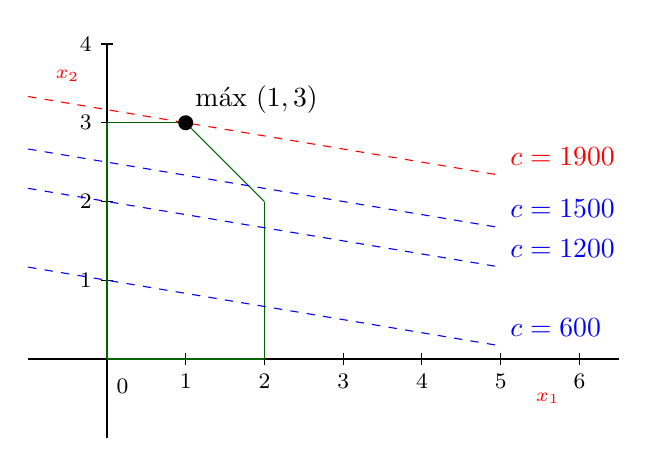
\begin{tikzpicture}[x=1.0cm,y=1.0cm]
\draw[color=black] (-1,0) -- (6.5,0);
\foreach \x in {1,2,3,4,5,6}
\draw[shift={(\x,0)},color=black] (0pt,2pt) -- (0pt,-2pt) node[below] {\footnotesize $\x$};
\draw[color=black] (0,-1) -- (0,4);
\foreach \y in {1,2,3,4}
\draw[shift={(0,\y)},color=black] (2pt,0pt) -- (-2pt,0pt) node[left] {\footnotesize $\y$};
\draw[color=black] (0pt,-10pt) node[right] {\footnotesize $0$};

\draw [color=qqwuqq] (0.,3.)-- (1.,3.);
\draw [color=qqwuqq] (1.,3.)-- (2.,2.);
\draw [color=qqwuqq] (2.,2.)-- (2.,0.);
\draw [color=qqwuqq] (2.,0.)-- (0.,0.);
\draw [color=qqwuqq] (0.,0.)-- (0.,3.);

\draw [domain=-1.:5, color = blue, dashed] plot(\x,{2.5-(\x/6)}) node[anchor=south west] {$c = 1500$};
\draw [domain=-1.:5, color = blue, dashed] plot(\x,{2-(\x/6)}) node[anchor=south west] {$c = 1200$};
\draw [domain=-1.:5, color = blue, dashed] plot(\x,{1-(\x/6)}) node[anchor=south west] {$c = 600$};
\draw [domain=-1.:5, color = red, dashed] plot(\x,{3.166666667-(\x/6)}) node[anchor=south west] {$c = 1900$};

\draw [fill=black] (1,3) circle(2.5pt) node [anchor = south west] {máx $(1,3)$};

\begin{scriptsize}
\draw[color=red] (5.6, -0.5) node {$x_1$};
\draw[color=red] (-0.5,3.6) node {$x_2$};
\end{scriptsize}
\end{tikzpicture}\end{center}\end{figura}
Luego nuestra solución óptima es producir un producto A y tres productos B.
\end{ejem}

Como hemos podido observar en el ejemplo anterior, la solución óptima ha sido alcanzada en un vértice del polígono que constituye la región factible. Esto se cumplirá, en general, siempre y cuando exista una solución, lo que denominamos como problema factible, y la región factible sea acotada. Esto es extendible a $n$ variables, en $\R^3$ la solución óptima se correspondería con un vértice del poliedro que constituye la región factible y en $\R^n$ con el politopo $n$-dimensional correspondiente.\\

Y es en esto en lo que consiste el método \textit{Símplex} que comentaremos más adelante, ideado por George Dantzig en 1947. Adelantaremos brevemente explicando que este algoritmo empieza en un vértice de la región factible, en el ejemplo anterior, por ejemplo el $(0,0)$ y continua estudiando los vértices vecinos hasta encontrar uno cuyos vecinos no sean una solución mejor que él. Ese vértice se corresponde con la solución óptima. En la \textit{figura 2.3} podemos ver un esquema iterativo de como actuaría el método \textit{Símplex} en el ejemplo anterior.
\begin{figura}\ \begin{center} \begin{tikzpicture}[x=1.0cm,y=1.0cm]
\foreach \x in {1,2}
\draw[shift={(\x,0)},color=black] (0pt,2pt) -- (0pt,-2pt) node[below] {\footnotesize $\x$};
\foreach \y in {1,2,3}
\draw[shift={(0,\y)},color=black] (2pt,0pt) -- (-2pt,0pt) node[left] {\footnotesize $\y$};
\draw[color=black] (0pt,-10pt) node {\footnotesize $0$};

\draw [color=gray] (0.,3.)-- (1.,3.);
\draw [color=gray] (1.,3.)-- (2.,2.);
\draw [color=gray] (2.,2.)-- (2.,0.);
\draw [color=gray] (2.,0.)-- (0.,0.);
\draw [color=gray] (0.,0.)-- (0.,3.);


\draw [fill=black] (0,0) circle(2.5pt) node [anchor = east] {0\euro};
\draw [fill=black] (2,0) circle(2.5pt) node [anchor = west] {200\euro};
\draw [fill=black] (2,2) circle(2.5pt) node [anchor = west] {1400\euro};
\draw [fill=black] (1,3) circle(2.5pt) node [anchor = south west] {máx 1900\euro};

\draw[-triangle 45] (1.1,0)-- (1.2,0);
\draw[-triangle 45] (2,1)-- (2,1.1);
\draw[-triangle 45] (1.5,2.5)-- (1.4,2.6);
\end{tikzpicture}\end{center} \end{figura}

\subsection{Problema de programación lineal de tres incógnitas (en $\R^3$)}
\begin{ejem} Veamos un segundo ejemplo. Imaginemos que la empresa del ejemplo anterior fabrica un nuevo producto C que les genera un beneficio de 1300\euro\ por unidad vendida. Las restricciones anteriores se mantienen: el producto A se limita a 2 unidades diarias, el B a 3, de nuevo sólo podemos fabricar 4 productos diarios y además queremos añadir la restricción $x_2+3x_3\leq 6$. Luego el planteamiento del problema sería el siguiente.\\
Función objetivo:
\[\mathrm{m\acute{a}x}\ z = 100x_1 + 600x_2+1300x_3\]
Restricciones:
\[x_1\leq 2\]
\[x_2\leq 3\]
\[x_1+x_2+x_3\leq 4\]
\[x_2+3x_3\leq 6\]
\[x_1,x_2,x_3\geq 0\]

Análogamente al ejercicio anterior, donde cada restricción representaba una recta, tenemos que ahora las restricciones representan un plano y la región factible generada es, como hemos comentado antes, un poliedro, como se muestra en la \textit{figura 2.4}. Así, para $n$ variables, cada restricción representa un hiperplano en $\R^n$ que a su vez generan un politopo $n$-dimensional correspondiente a la región factible.

De igual modo, podemos asignar un valor $c$ de manera que el plano $z(x_1,x_2,x_3)=c$ se corresponde con los puntos $(x_1,x_2,x_3)$ cuyo beneficio es $c$. De nuevo, podríamos trazar distintos planos paralelos para distintos valores de $c$ para intuir cuál es la solución óptima.

Para finalizar, comentamos que para este problema tiene como solución óptima los valores $x_1=0,x_2=3,x_3=1$.
\begin{figura}\ \begin{center} 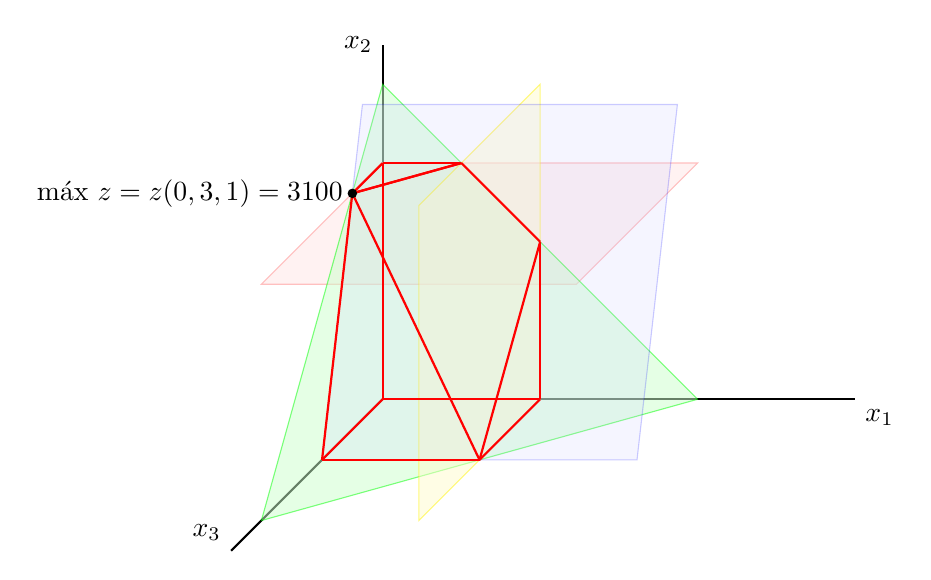
\begin{tikzpicture}
\draw[thick](0,0,0) -- (6,0,0) node[anchor=north west] {$x_1$};
\draw[thick] (0,0,0) -- (0,4.5,0) node[anchor=east] {$x_2$};
\draw[thick] (0,0,0) -- (0,0,5) node[anchor=south east] {$x_3$};

\filldraw[draw=pink,fill=pink!20] (0,3,0) -- (4,3,0) -- (4,3,4) -- (0,3,4) -- (0,3,0);
\filldraw[draw=green,fill=green!20, opacity=0.5] (4,0,0) -- (0,0,4) -- (0,4,0) -- (4,0,0);
\filldraw[draw=yellow,fill=yellow!20, opacity=0.5] (2,0,0) -- (2,0,4) -- (2,4,4) -- (2,4,0) -- (2,0,0);
\filldraw[draw=blue,fill=blue!20, opacity=0.2] (0,0,2) -- (4,0,2) -- (4,4,0.667) -- (0,4,0.667) --(0,0,2);

\draw[thick, red] (0,0,0) -- (2,0,0);
\draw[thick, red] (0,0,0) -- (0,3,0);
\draw[thick, red] (0,3,0) -- (1,3,0);
\draw[thick, red] (1,3,0) -- (2,2,0);
\draw[thick, red] (2,2,0) -- (2,0,0);
\draw[thick, red] (0,0,0) -- (0,0,2);
\draw[thick, red] (0,0,2) -- (2,0,2);
\draw[thick, red] (2,0,2) -- (2,0,0);
\draw[thick, red] (0,0,2) -- (0,3,1);
\draw[thick, red] (0,3,1) -- (0,3,0);
\draw[thick, red] (0,3,1) -- (2,0,2);
\draw[thick, red] (2,0,2) -- (2,2,0);
\draw[thick, red] (0,3,1) -- (1,3,0);

\draw[thick, red] (0,3,1) -- (1,3,0);

\draw [fill=black] (0,3,1) circle(1.5pt) node[anchor=east]{máx $z=z(0,3,1)=3100$\euro};

            

\end{tikzpicture}\end{center} \end{figura}
\end{ejem}